\chapter{Rešerše}
\label{0-reserse}

Tarifní pásma Pražské integrované dopravy jsou mimo jiné publikována jako shapefile 
\footnote{formát vektorového datového úložiště Esri pro ukládání umístění,
tvaru a atributů geografických prvků \cite{shapefile}}
na portálu \textit{opendata hlavního města Prahy} \cite{opendata}. Tento shapefile
obsahuje vektorové vrstvy polygonů.

První myšlenkou, jak se přiblížit k takovým polygonům bylo vytvoření linií mezi jednotlivými zastávkami.
K tomu slouží takzvaná triangulace, která vytvoří trojúhelníky bezi body, kde uvnitř těchto trojuhelníků  
už neleží žádné body a každý trojúhelník má vždy společnou jednu hranu. 

Takové triangulace se používají v kartografii, tak v GIS, v Dálkovém průzkumu země,
počítačové grafice, při analýze vlastností a struktury materiálů, plánování pohybu robotů
nebo při modelování přírodních jevů. \cite{bayer-delaunay}

Existuje více druhů triangulací, které využívají vždy jinou metodu konstrukce
a mají rozdílný výpočetní stupeň složitosti. 

Hladová (Greedy) triangulace se snaží vytvářet trojúhelníky s nejkratšími stranami,
které nesplňují žádnou speciální geometrickou podmínku. Její realizace je jednoduchá,
avšak důsledek toho jsou často tvarově nepěkné nebo nevhodné trojúhelníky. Má velkou výpočetní
složitost \(O(n^3)\), lze optimalizovat na \(O(n^2 \log(n))\) a v kartografii se 
nepříliš používá. \cite{vanicek}

\begin{figure}[H] \centering
    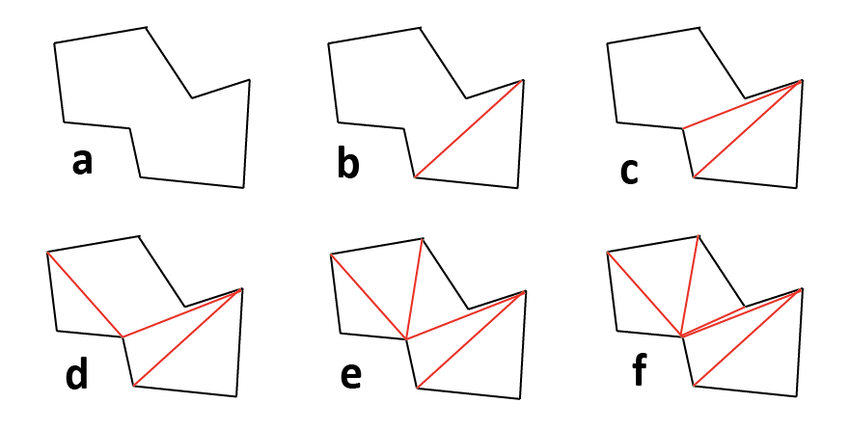
\includegraphics[width=400pt]{./pictures/triangulace-greedy.png}
    \caption[Ilustrace Greedy triangulace]{Ilustrace Greedy triangulace \cite{triangulace-greedy}}
	\label{fig:triangulace-greedy}              
\end{figure}

Další triangulací je tzv. Delaunay triangulace, která je nejčastěji používaná.
Delaunay triangulací se rozumí vytváření liniových spojnic bodů mez jednotlivými body, které si jsou sobě nejblíž,
za pomocí opsaných kružnic. Delaunay triangulace má několik vlastností. Jednou z nich je například,
že uvnitř kružnice k opsané libovolnému trojúhelníku neleží žádný jiný bod.
Zároveň Delaunay triangulace je jednoznačná, pokud žádné čtyři body neleží na kružnici.
Na rozdíl od Greedy triangulace nehodnotí kritérium délky hran. Díky maximalizaci minimálních
úhlů vytváří takové trojúhelníky, které se nejvíc blíží k rovnostranným trojúhelníkům, 
což znamená, že se snaží eliminovat trojúhelníky, které jsou ostroúhlé.

Pro výtváření konstrukce Delaunay triangulace jsou k dispozici různé algoritmy: lokální prohazování, 
inkrementální konstrukce, inkrementální vkládání, rozděl a panuj nebo sweep line. \cite{bayer-delaunay}

\begin{figure}[H] \centering
    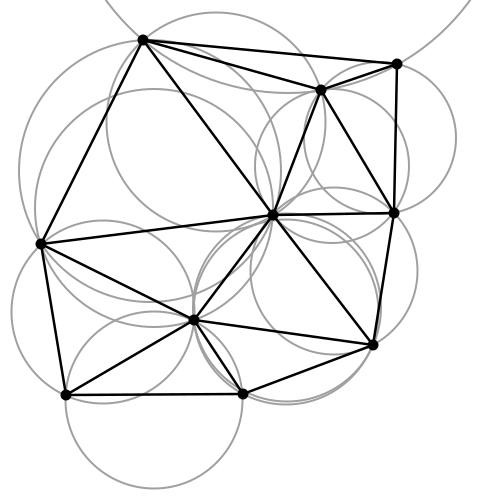
\includegraphics[width=280pt]{./pictures/triangulace-delaunay.png}
    \caption[Ilustrace Delaunay triangulace]{Ilustrace Delaunay triangulace \cite{triangulace-delaunay}}
	\label{fig:triangulace-delaunay}              
\end{figure}

Poté existuje triangulace s minimální hmotností (anglicky Minimum Weight Triangulation, zkráceně MWT),
která má minimální celkovou délku hran. MWT je nejlepší triangulace pro interpolaci trojrozměrných oblastí,
tudíž se pro tvorbu 2D tarifních pásem úplně nehodí.

% Konvexní obálka - definice, metody konstrukce

% Konkávní obálka - definice, metody konstrukce

Tarifní pásma zasahují tam, kde nejsou žádné zastávky. Pro takové vyplnění plochy
mezi zastávkami a pro místa, kde zastávky nejsou (většinou na krajích zón) není triangulace, konvexní nebo konkávní 
obálka úplně vhodná. Pro takový problém bylo další myšlenkou použít teselaci, což je vyplnění roviny pomocí jednoho
nebo více geometrických útvarů vzájemně spojených, bez překrývú a mezer. Triangulace, konvexní nebo konkávní 
obálka se mohou hodit při dalších krocích výpočtu.

Nejpoužívanější teselací v oblastí GIS je Voronoi diagram, někdy nazývána Voroného teselace, Voroného dekompozice,
Thiessenovy polygony nebo Dirichletova teselace, což je způsob rozkladu 
metrického prostoru určený vzdálenostmi k dané nespojité množině bodů v prostoru.
V našem případě se bude řešit Voronoi diagram ve 2D prostoru, tedy v rovině.

Takže na vstupu Voronoi diagramu je nějaká množina bodů a výstupem je Voronoi diagram, 
což představuje takovou množinu buněk, pro které bude platit, že každý bod
\textit{q} nálěžící množině \textit{V(p\textsubscript{i})} je blíže k bodu
\textit{p\textsubscript{i}} než k jakémukoliv
bodu \textit{p\textsubscript{j}} náležící množině \textit{P}.  \cite{bayer-voronoi}

Pro lepší chápání Voronoi diagramů je potřeba si vysvětlit její terminologii.
Vstupní množinu bodů nazýváme generátory, každý bod generuje jednu Voronoi buňku. V 
terminologii GIS se hovoří o tzv. Voronoi polygony. Tyto Voronoi buňky jsou tvořeny hranami,
které spojují dva Voronoi vrcholy. Dohromady tyto Voronoi buňky tvoří Voronoi diagram.  

\begin{figure}[H] \centering
    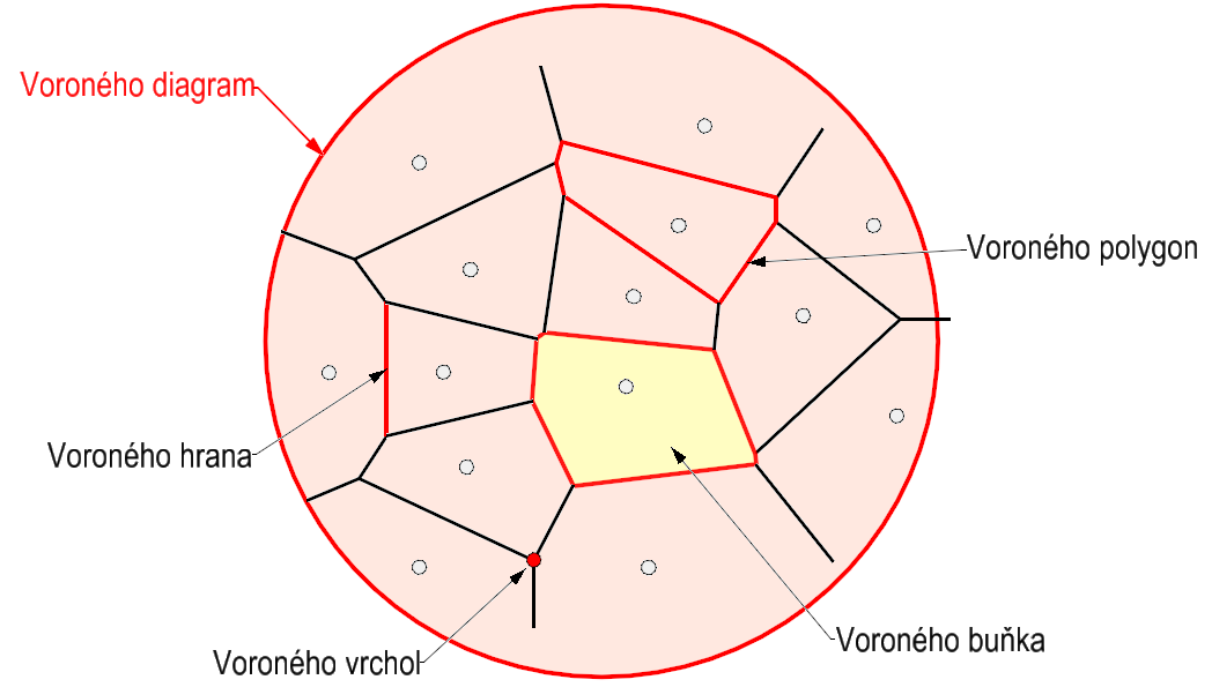
\includegraphics[width=400pt]{./pictures/bayer-voronoi-terminologie.png}
    \caption[Terminologie Voronoi diagramu]{Terminologie Voronoi diagramu \cite{bayer-voronoi}}
	\label{fig:bayer-voronoi-terminologie}              
\end{figure}

Voronoi diagramy mají své vlastnosti, které jsou důležité pro jejich tvorbu. V následujících
odrážkách jsou doslovně citována jejih znění z prezentace pana doc. Ing. Tomáše Bayera, Ph.D.

\begin{itemize}
\item Voronoi diagram \textit{V(P)} je planárním grafem.
\item Vrchol q Voronoi buňky \textit{\{V(p\textsubscript{i})} je průnikem 3 hran, právě když je \textit{V(P)} nedegenerovaný.
\item Pokud \textit{p\textsubscript{i}} náležící \textit{H(P)}, pak je \textit{V(p\textsubscript{i})}  otevřený. 
\item Pro každý bod \textit{p\textsubscript{i} náležící P} je \textit{V(P)} konvexní. 
\item Bod \textit{p\textsubscript{i}} je nejbližším bodem bodu \textit{p}
jestliže \textit{p} náleží \textit{\{V(p\textsubscript{i})}.
\item Každá strana \textit{q\textsubscript{i}q\textsubscript{j}}, \(i \neq j\),
je sdílena právě dvěma sousedními buňkami \textit{V(p)}. 
\item Bod q je vrcholem \textit{V(p)}, pokud existuje kružnice \textit{k(q,r)} procházející třemi
nebo více generátory \textit{p\textsubscript{i}}, \textit{p\textsubscript{j}},
\textit{p\textsubscript{k}}, a neobsahuje žádný další bod P (spojitost s \textit{DT(P)}). 
\item Kružnici \textit{k(q,r)} označujeme jako největší prázdnou kružnici ze všech prázdných kružnic se středem v bodě \textit{q}. 
\item Průměrné množství Voronoi hran ve Voronoi polygonu nepřekročí hodnotu 6. 
\item Vztah mezi počtem bodů \textit{n}, počtem hran \textit{n\textsubscript{h}}
a počtem trojúhelníků \textit{n\textsubscript{t}} teselace \textit{V(P)}:
\[ n_h \leq 3n-6\]
\[ n_t \leq 2n−5\]
\item Voronoi diagram \textit{V(P)} představuje ortografickou projekci stěn
mnohostěnu tvořeného průsečnicemi všech polorovin \textit{A\textsubscript{i}} do roviny \textit{xy}. 
\item Nechť bod \textit{p\textsubscript{i}\textsuperscript{*}} i představuje
ortografický průmět bodu \textit{p\textsubscript{i}} na povrch paraboloidu daného rovnicí:
\[ z = x^2 + y^2 \]
   
\end{itemize}

\begin{figure}[H] \centering
    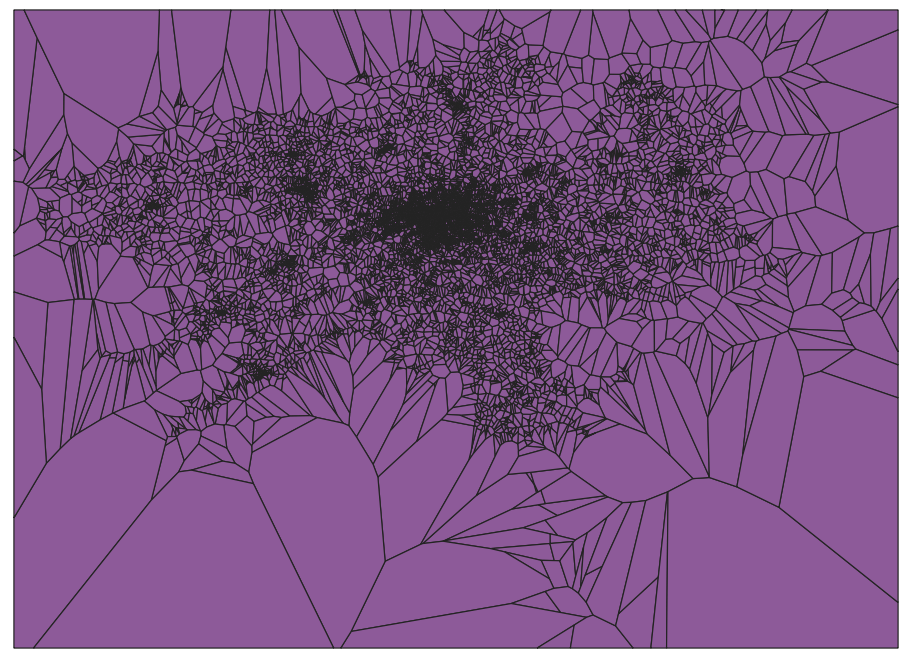
\includegraphics[width=400pt]{./pictures/voronoi.png}
    \caption[Voroného polygony]{Voroného polygony}
	\label{fig:voronoi}              
\end{figure}   

Voronoi diagram má jistý vztah s Delaunay triangulací. Hraniční vstupní body
Voronoi diagramu po spojení Delaunay triangulací tvoří konvexní obálku.
Středy kružnic opsaných trojúhelníků Delaunay triangulace představují úzlové body
Voronoi diagramu.

Pro konstrukci Voronoi diagramu existují různé metody. Konstrukce lze v praxi tvořit přímo nebo nepřímo.
Pro přímou konstrukci jsou tu metody Inkrementální konstrukce, Sweep line algoritmus a
Rozděl a panuj. Nepřímá konstrukce je vytvářena přes Delaunay triangulaci skrz spojení středů
kružnic opsaných trojúhelníků a bývá nejpoužívanější. 

Využití Voronoi diagramů v oblasti GIS je široké. Například tzv. poštovní problém
pomáhá při návrhu nových supermarkétů, stanic MHD či polohy nových nemocnic.
Další využití jsou například nalezení všech sousedů, převod bodových údajů na plošné
nebo klasifikace dat.

 